\documentclass[12pt,a4paper]{article}%
%Options -- Point size:  10pt (default), 11pt, 12pt
%        -- Paper size:  letterpaper (default), a4paper, a5paper, b5paper
%                        legalpaper, executivepaper
%        -- Orientation  (portrait is the default)
%                        landscape
%        -- Print size:  oneside (default), twoside
%        -- Quality      final(default), draft
%        -- Title page   notitlepage, titlepage(default)
%        -- Columns      onecolumn(default), twocolumn
%        -- Equation numbering (equation numbers on the right is the default)
%                        leqno
%        -- Displayed equations (centered is the default)
%                        fleqn (equations start at the same distance from the right side)
%        -- Open bibliography style (closed is the default)
%                        openbib
% For instance the command
%           \documentclass[a4paper,12pt,leqno]{article}
% ensures that the paper size is a4, the fonts are typeset at the size 12p
% and the equation numbers are on the left side

% Tabelas
\usepackage{multirow}

% Símbolos Matemáticos
\usepackage{amsmath}
\usepackage{amsfonts}
\usepackage{amssymb}
\usepackage{bm}
\usepackage{commath}

% Figuras
\usepackage{graphicx}

%\usepackage{wrapfig}
\usepackage{float}

% Língua e acentos
\usepackage[brazil]{babel}
\usepackage[utf8]{inputenc}
\usepackage[T1]{fontenc}

% Espaçamento
\usepackage[top=3cm, bottom=2cm, left=2cm, right=2cm]{geometry}
\usepackage{indentfirst}

\usepackage{afterpage}
\newcommand\blankpage{%
    \null
    \thispagestyle{empty}%
    \addtocounter{page}{-1}%
    \newpage}

% Lista de códigos
\usepackage{listings}                   % para formatar código-fonte
\lstset{numbers=left, numberstyle=\tiny, stepnumber=1, numbersep=5pt, basicstyle=\scriptsize , frame=trbl}

%\usepackage{enumerate}
\usepackage{enumitem}

% Latexdraw
%\usepackage[usenames,dvipsnames]{pstricks}
%\usepackage{epsfig}
%\usepackage{pst-grad} % For gradients
%\usepackage{pst-plot} % For axes

%------------------------------------------------------------------------------

\begin{document}

\begin{titlepage}
\begin{center}
\begin{figure}[h]

\includegraphics[scale=0.76]{Imagens/topdotitulo.png}
\end{figure}
\rule{\columnwidth}{1.5mm}
\

\large David Maykon Krepsky Silva\\
\large Daniel Galbes Bassanezi\\

\vspace{4cm}
{\bf \Large Modulador AM}
\vspace{3.5cm}

\begin{flushright}
Data de realização do experimento:\\
20 de agosto de 2015\\
Série/Turma:\\
1000/1011\\
Prof. Dr. Jaime Laelson Jacob 
\end{flushright}

\vspace{3.2cm}
\today

\rule{\columnwidth}{1.3mm}
\end{center}
\end{titlepage}

\newpage
\begin{abstract}
\addcontentsline{toc}{section}{Resumo}

Neste trabalho foi realizado o estudo teórico e a simulação de dois circuitos moduladores AM DSB, de forma a comprovar, em simulação computacional, a validade e as limitações do projeto de moduladores, utilizando o modelo de pequenos sinais. As topologias utilizadas empregam transistores, para o primeiro circuito, e um diodo, para o segundo. Foi observado que, embora o circuito com diodo tenha um número pequeno de componentes, resultando em baixo custo, o mesmo possui um fator de mérito menor que o do modulador transistorizado.
\end{abstract}

\newpage
\tableofcontents

\newpage
\section{Introdução}
Introdução ao experimento
\newpage
\section{Teoria}
\subsection{Modulação AM DSB}
A modulação em amplitude consiste em modificar a amplitude de um sinal de frequência constante, chamado de portadora, a partir de um sinal modulante (informação). O termo DSB significa \textit{double side band}, pois o espectro do sinal modulado possui tanto a banda positiva quanto a banda negativa do sinal modulante.

O sinal modulado em AM DSB pode ser representado matematicamente pela equação

\begin{equation}
s(t) = A_c[1+\gamma f(t)]cos(w_c t).
\label{e_am}
\end{equation}

Onde $f(t)$ é o sinal de informação, $A_c$ é a amplitude, $\gamma$ é o índice de modulação e $w_c$ é a frequência angular da portadora.

Sendo 
\[ f(t) = cos(w_m t), \]

temos que
\begin{equation}
s(t) = A_c  \bigg \{ sen(w_c t) + \frac{\gamma}{2}sen(w_c + w_m)t + \frac{\gamma}{2}sen(w_c - w_m)t \bigg  \} .
\label{e_amdsb}
\end{equation}

A transformada de Fourier do sinal da equação \ref{e_amdsb} (mostrada na figura \ref{f_fourier_am_dsb} ) é 
\[
F(s) = \mathfrak{F} \big \{ f(t) \big \} = A_c \delta (s - w_c) + A_c \frac{\gamma}{2}\delta(w_c  + w_m) + A_c \frac{\gamma}{2}\delta(w_c  - w_m)
\]

\begin{figure}[H]
    \centering
    \caption{Modulo do espectro complexo de Fourier da modulação AM DSB com sinal modulante cossenoidal.}
    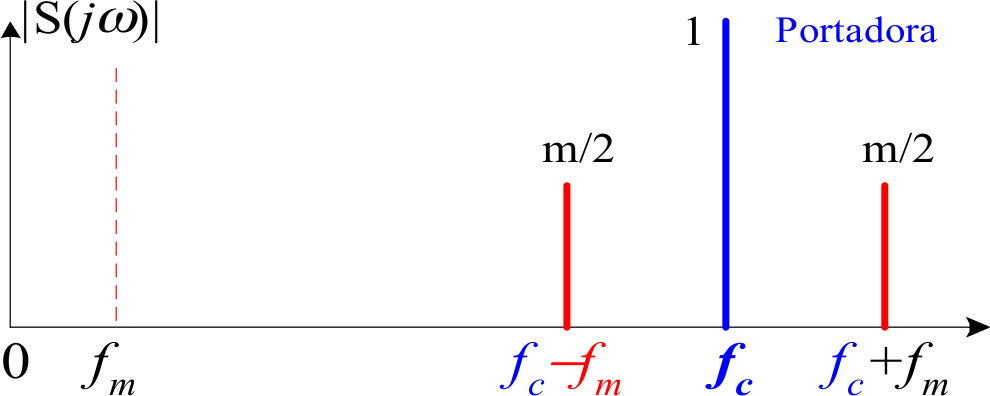
\includegraphics[scale=0.3]{Imagens/fourier_am_dsb.png}
    \label{f_fourier_am_dsb}
\end{figure}


\subsection{Medida do índice de modulação $\bm{\gamma}$}
O índice de modulação ($\gamma$) pode ser obtido através da equação \ref{e_gamma}, onde os valores de \textit{a} e \textit{b} podem ser definidos de duas maneiras.

\begin{equation}
\gamma = \frac{a - b}{a + b}
\label{e_gamma}
\end{equation}

\subsubsection{Método 1}
No método 1, o sinal modulado é colocado no eixo Y e o tempo é colocado no eixo X. O valor de \textit{a} é dado pela amplitude de pico a pico do sinal modulado quando $f(t)$ é máximo e o valor de \textit{b} é dado pelo valor de pico a pico para quando o sinal  $f(t)$ é mínimo. A figura \ref{f_gamma1} mostra um exemplo do cálculo.

\begin{figure}[H]
\centering
\caption{Exemplo para o calculo de $\gamma$, com \textit{a} = 3, \textit{b} = 1 e $\gamma$ = 0.5.}
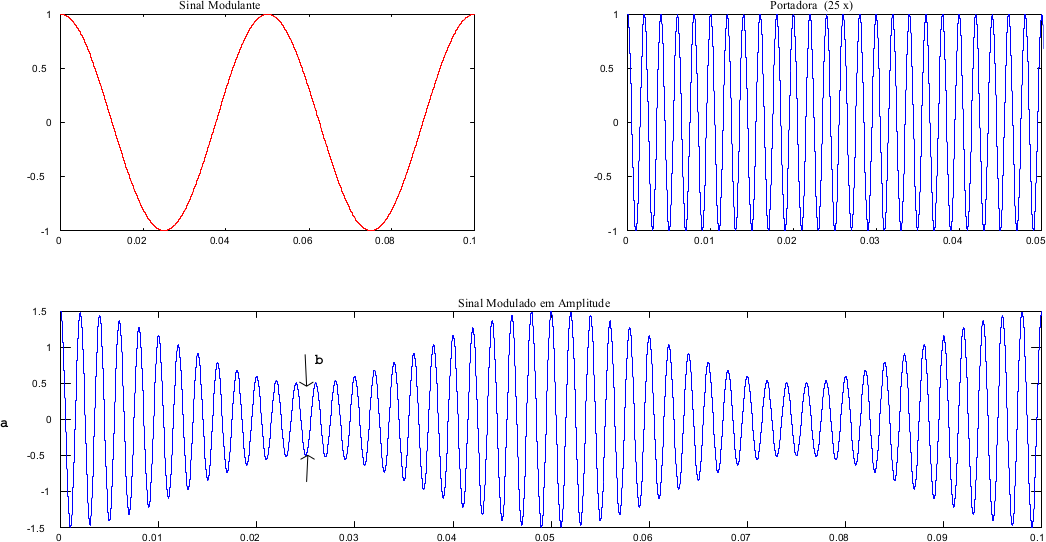
\includegraphics[scale=0.4]{Imagens/gamma1.png}
\label{f_gamma1}
\end{figure}

\subsubsection{Método 2}

No método 2, o sinal modulado é colocado no eixo Y e o sinal modulante é colocado no eixo X. O valor de \textit{a} é dado pela amplitude de pico a pico do da parte mais baixa da figura e o valor de \textit{b} é dado pelo valor de pico a pico mais alto. A figura \ref{f_gamma2} mostra um exemplo do cálculo.

\begin{figure}[H]
    \centering
    \caption{Exemplo para o calculo de $\gamma$, com \textit{a} = 0.2, \textit{b} = 0.6 e $\gamma$ = 0.5.}
    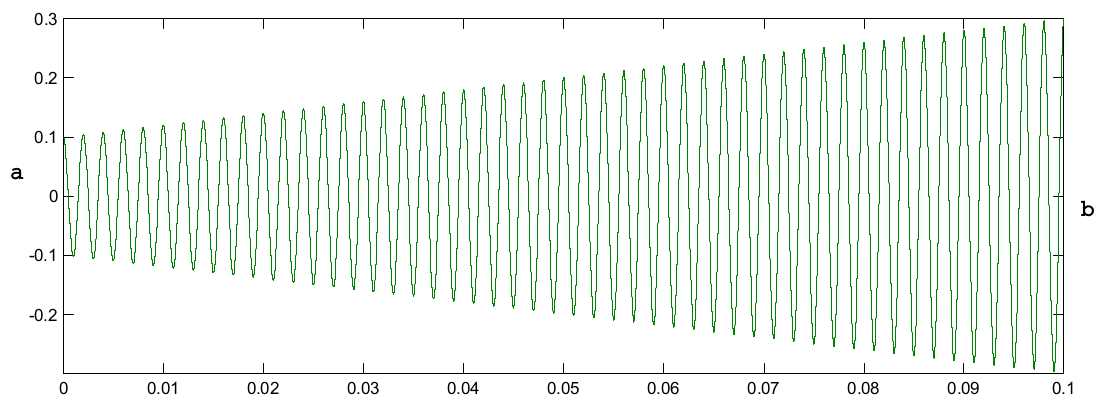
\includegraphics[scale=0.4]{Imagens/gamma2.png}
    \label{f_gamma2}
\end{figure}

O método 2 é preferível, pois evidencia a linearidade do modulador, independente da forma de onda do sinal modulante. Porém, quando são introduzidas distorções no sinal modulado, o método 1 deve ser utilizado.

\subsection{Circuitos moduladores}
Abaixo são apresentadas duas topologias de circuito modulador AM DSB, uma utilizando transistores e a outra empregando um único diodo.

\subsubsection{Modulador série}

A figura \ref{f_mod_am_serie} apresenta a configuração do circuito utilizado em um modulador AM/DSB série.
Os moduladores série modificam diretamente a amplitude do sinal de RF, assim, evitando distorções na frequência do sinal modulado.

O transistor Q1 acopla sinal de informação ao coletor do amplificador de RF de saída, Q2, evitando a necessidade de um transformador, o que reduz o custo e o tamanho do circuito.

O filtro passa-baixas composto por $C_{f1}$ , $C_{f2}$, $C_p$ e $L_f$ atua, também, como um circuito LC paralelo sintonizado na frequência da portadora ($f_c$) e como uma rede $\pi$ casadora de impedância.

\begin{figure}[H]
    \centering
    \caption{Circuito do modulador série.}
    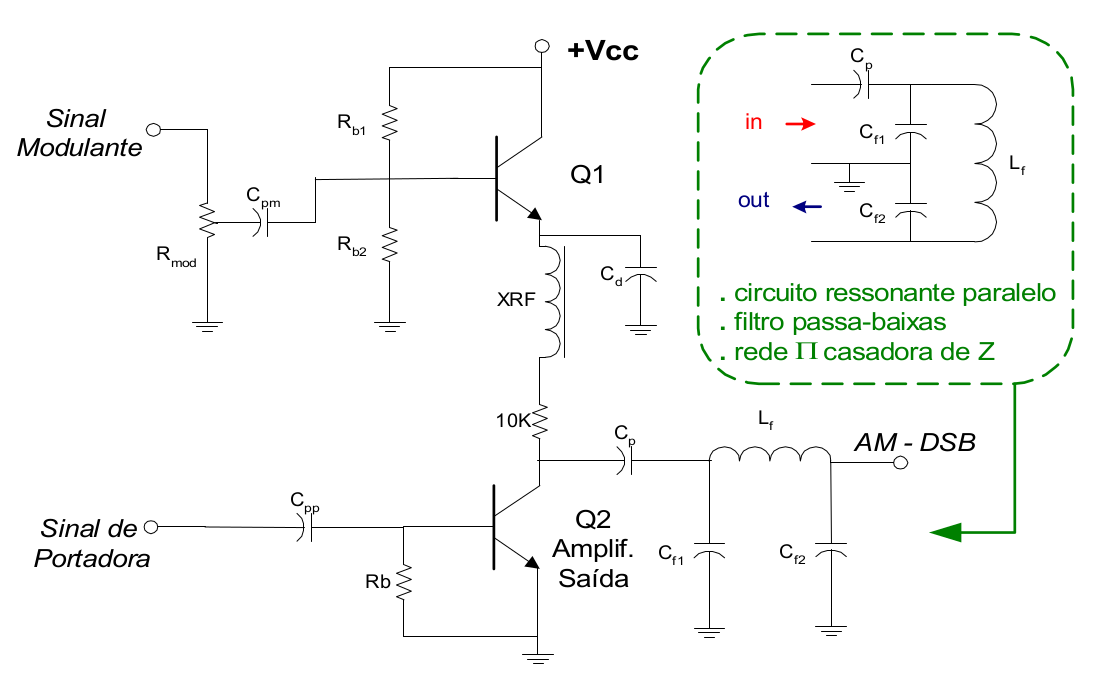
\includegraphics[scale=0.4]{Imagens/mod_am_serie.png}
    \label{f_mod_am_serie}
\end{figure}

\subsubsection{Modulador a diodo}

A figura \ref{f_mod_am_diodo} apresenta a configuração do circuito utilizado em um modulador AM/DSB simples.
Os moduladores série modificam diretamente a amplitude do sinal de RF, assim, evitando distorções na frequência do sinal modulado.

\begin{figure}[H]
    \centering
    \caption{Circuito do modulador a diodo.}
    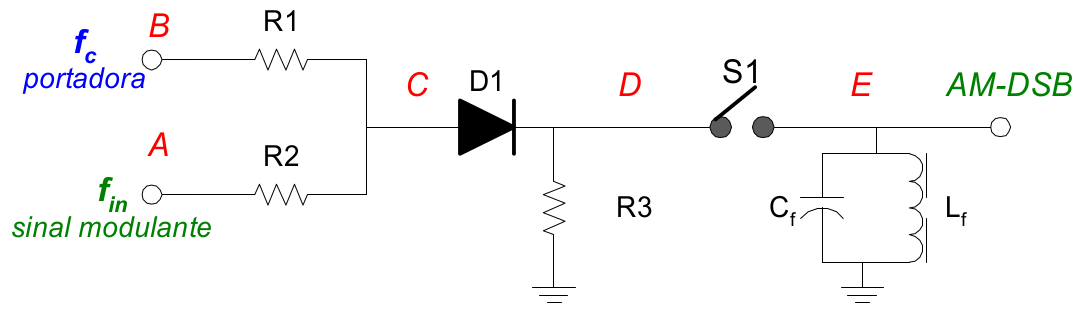
\includegraphics[scale=0.4]{Imagens/mod_am_diodo.png}
    \label{f_mod_am_diodo}
\end{figure}

A chave S1, quando o circuito está em operação, fica normalmente fechada.
O filtro passa-faixa composto por $C_f$ e $L_f$ é sintonizado em $f_c$. Assim, para cada semi-ciclo positivo de $f_c$ o circuito ressonante paralelo produz um semi-ciclo negativo, resultando à saída a forma de
onda E da figura \ref{f_mod_am_diodo_ex}.



\begin{figure}[H]
    \centering
    \caption{Formas de onda em um modulador a diodo.}
    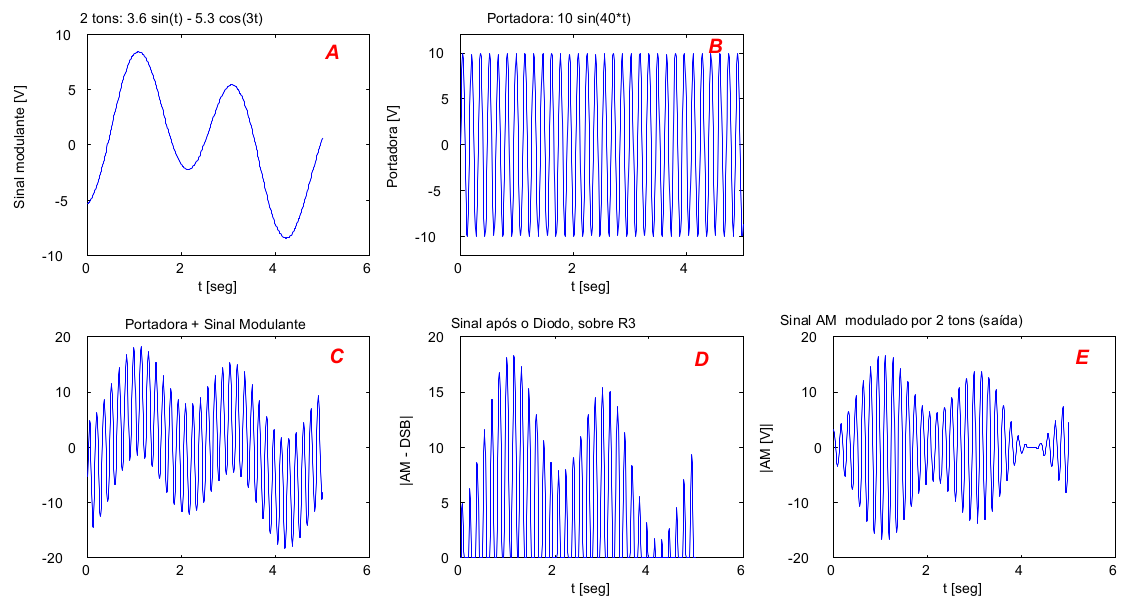
\includegraphics[scale=0.4]{Imagens/mod_am_diodo_ex.png}
    \label{f_mod_am_diodo_ex}
\end{figure}
\newpage
\section{Metodologia Experimental}

\subsection{Materiais}
O material utilizado foi:
\begin{itemize}
    \item Computador.
    \item Software Orcad.
    
\end{itemize}
O experimento foi dividido em duas partes, sendo a parte 1 para o modulador série e a parte 2 com o modulador a diodo.

\subsubsection{Modulador série}
Para execução da parte 1 do experimento, faz-se necessário executar os seguintes passos (com base no circuito da figura \ref{f_sch_mod_am_serie}):

\begin{itemize}
    \item montar o circuito mostrado na figura \ref{f_sch_mod_am_serie} no software Orcad;
    \item utilizar um sinal senoidal de 200Hz (2 $V_{pp}$) como modulante e um sinal de 110kHz como portadora;
    \item Obter o índice de modulação $\gamma$ do circuito através do método 1 e do método 2;
    \item verificar quais são os limites para $\gamma$;
    \item caso seja possível obter índice m > 1,observe o que ocorre com sinal quando se utiliza o método 2. É possível aplicar este método na avaliação de índices de modulação maiores que 100\%?;
    \item determinar o fator de mérito do modulador.
    \item Modificar o valor do circuito LC de modo a obter o dobro do fator de mérito;
    \item analisar o sinal de saída no domínio da frequência;
    \item como é possível reduzir eventuais componentes de frequência espúrias à saída?
\end{itemize}

\begin{figure}[H]
    \centering
    \caption{Modulador série.}
    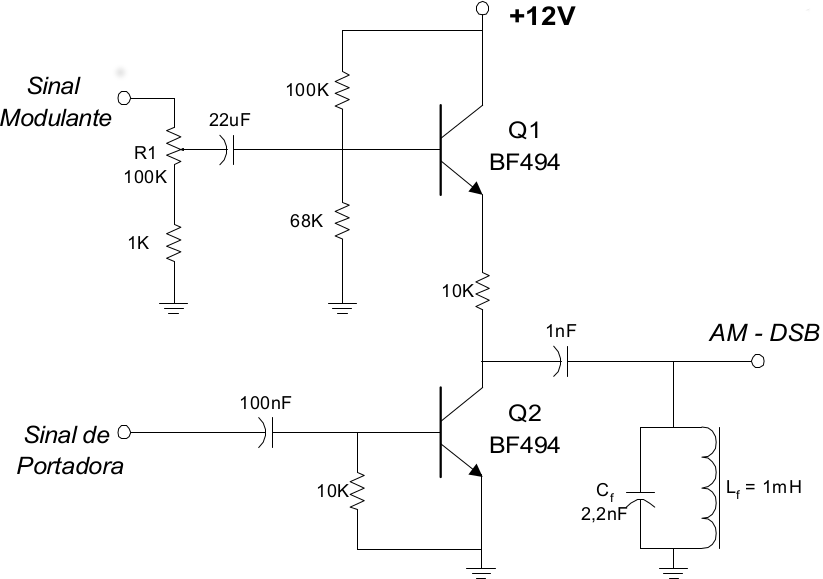
\includegraphics[scale=0.4]{sch_mod_am_serie.png}
    \label{f_sch_mod_am_serie}
\end{figure}

\subsubsection{Modulador a diodo}
Para execução da parte 2 do experimento, faz-se necessário executar os seguintes passos (com base no circuito da figura \ref{f_sch_mod_am_diodo}):

\begin{itemize}
    \item montar o circuito mostrado na figura \ref{f_sch_mod_am_diodo} no software Orcad;
    \item utilizar um sinal senoidal de 2kHz (2 $V_{pp}$) como modulante e um sinal de 110kHz (5 $V_{pp}$) como portadora;
    \item calcular o valor de $L_1$ e $C_1$ de modo que a frequência de ressonância fique próxima de $f_c$.
    \item verificar se o sinal modulante é banda estreita;
    \item Obter o índice de modulação $\gamma$ do circuito através do método 1 e do método 2;
    \item determinar o fator de mérito do modulador.
    \item analisar o sinal de saída no domínio da frequência;
\end{itemize}

\begin{figure}[H]
    \centering
    \caption{Modulador a diodo.}
    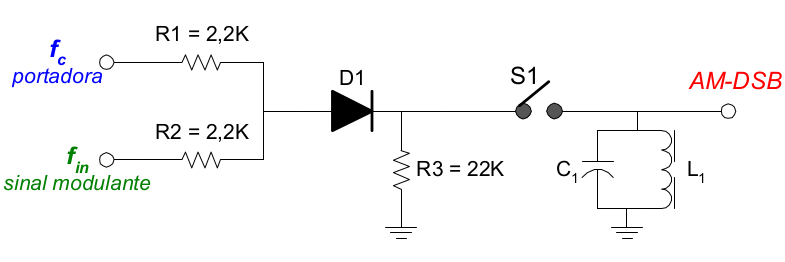
\includegraphics[scale=0.5]{sch_mod_am_diodo.png}
    \label{f_sch_mod_am_diodo}
\end{figure}

\newpage
\section{Resultados}

\subsection{Método 1: Transmissão de pelo menos duas formas de onda de dados com a metade da taxa}

Para o método 1, primeiramente foi realizada a montagem, de acordo com a figura \ref{fig:montagem}-a, conforme mostra a figura \ref{fig:montagem1}.

\begin{figure}[H]
  \centering
  \caption{Montagem para o primeiro experimento.}
  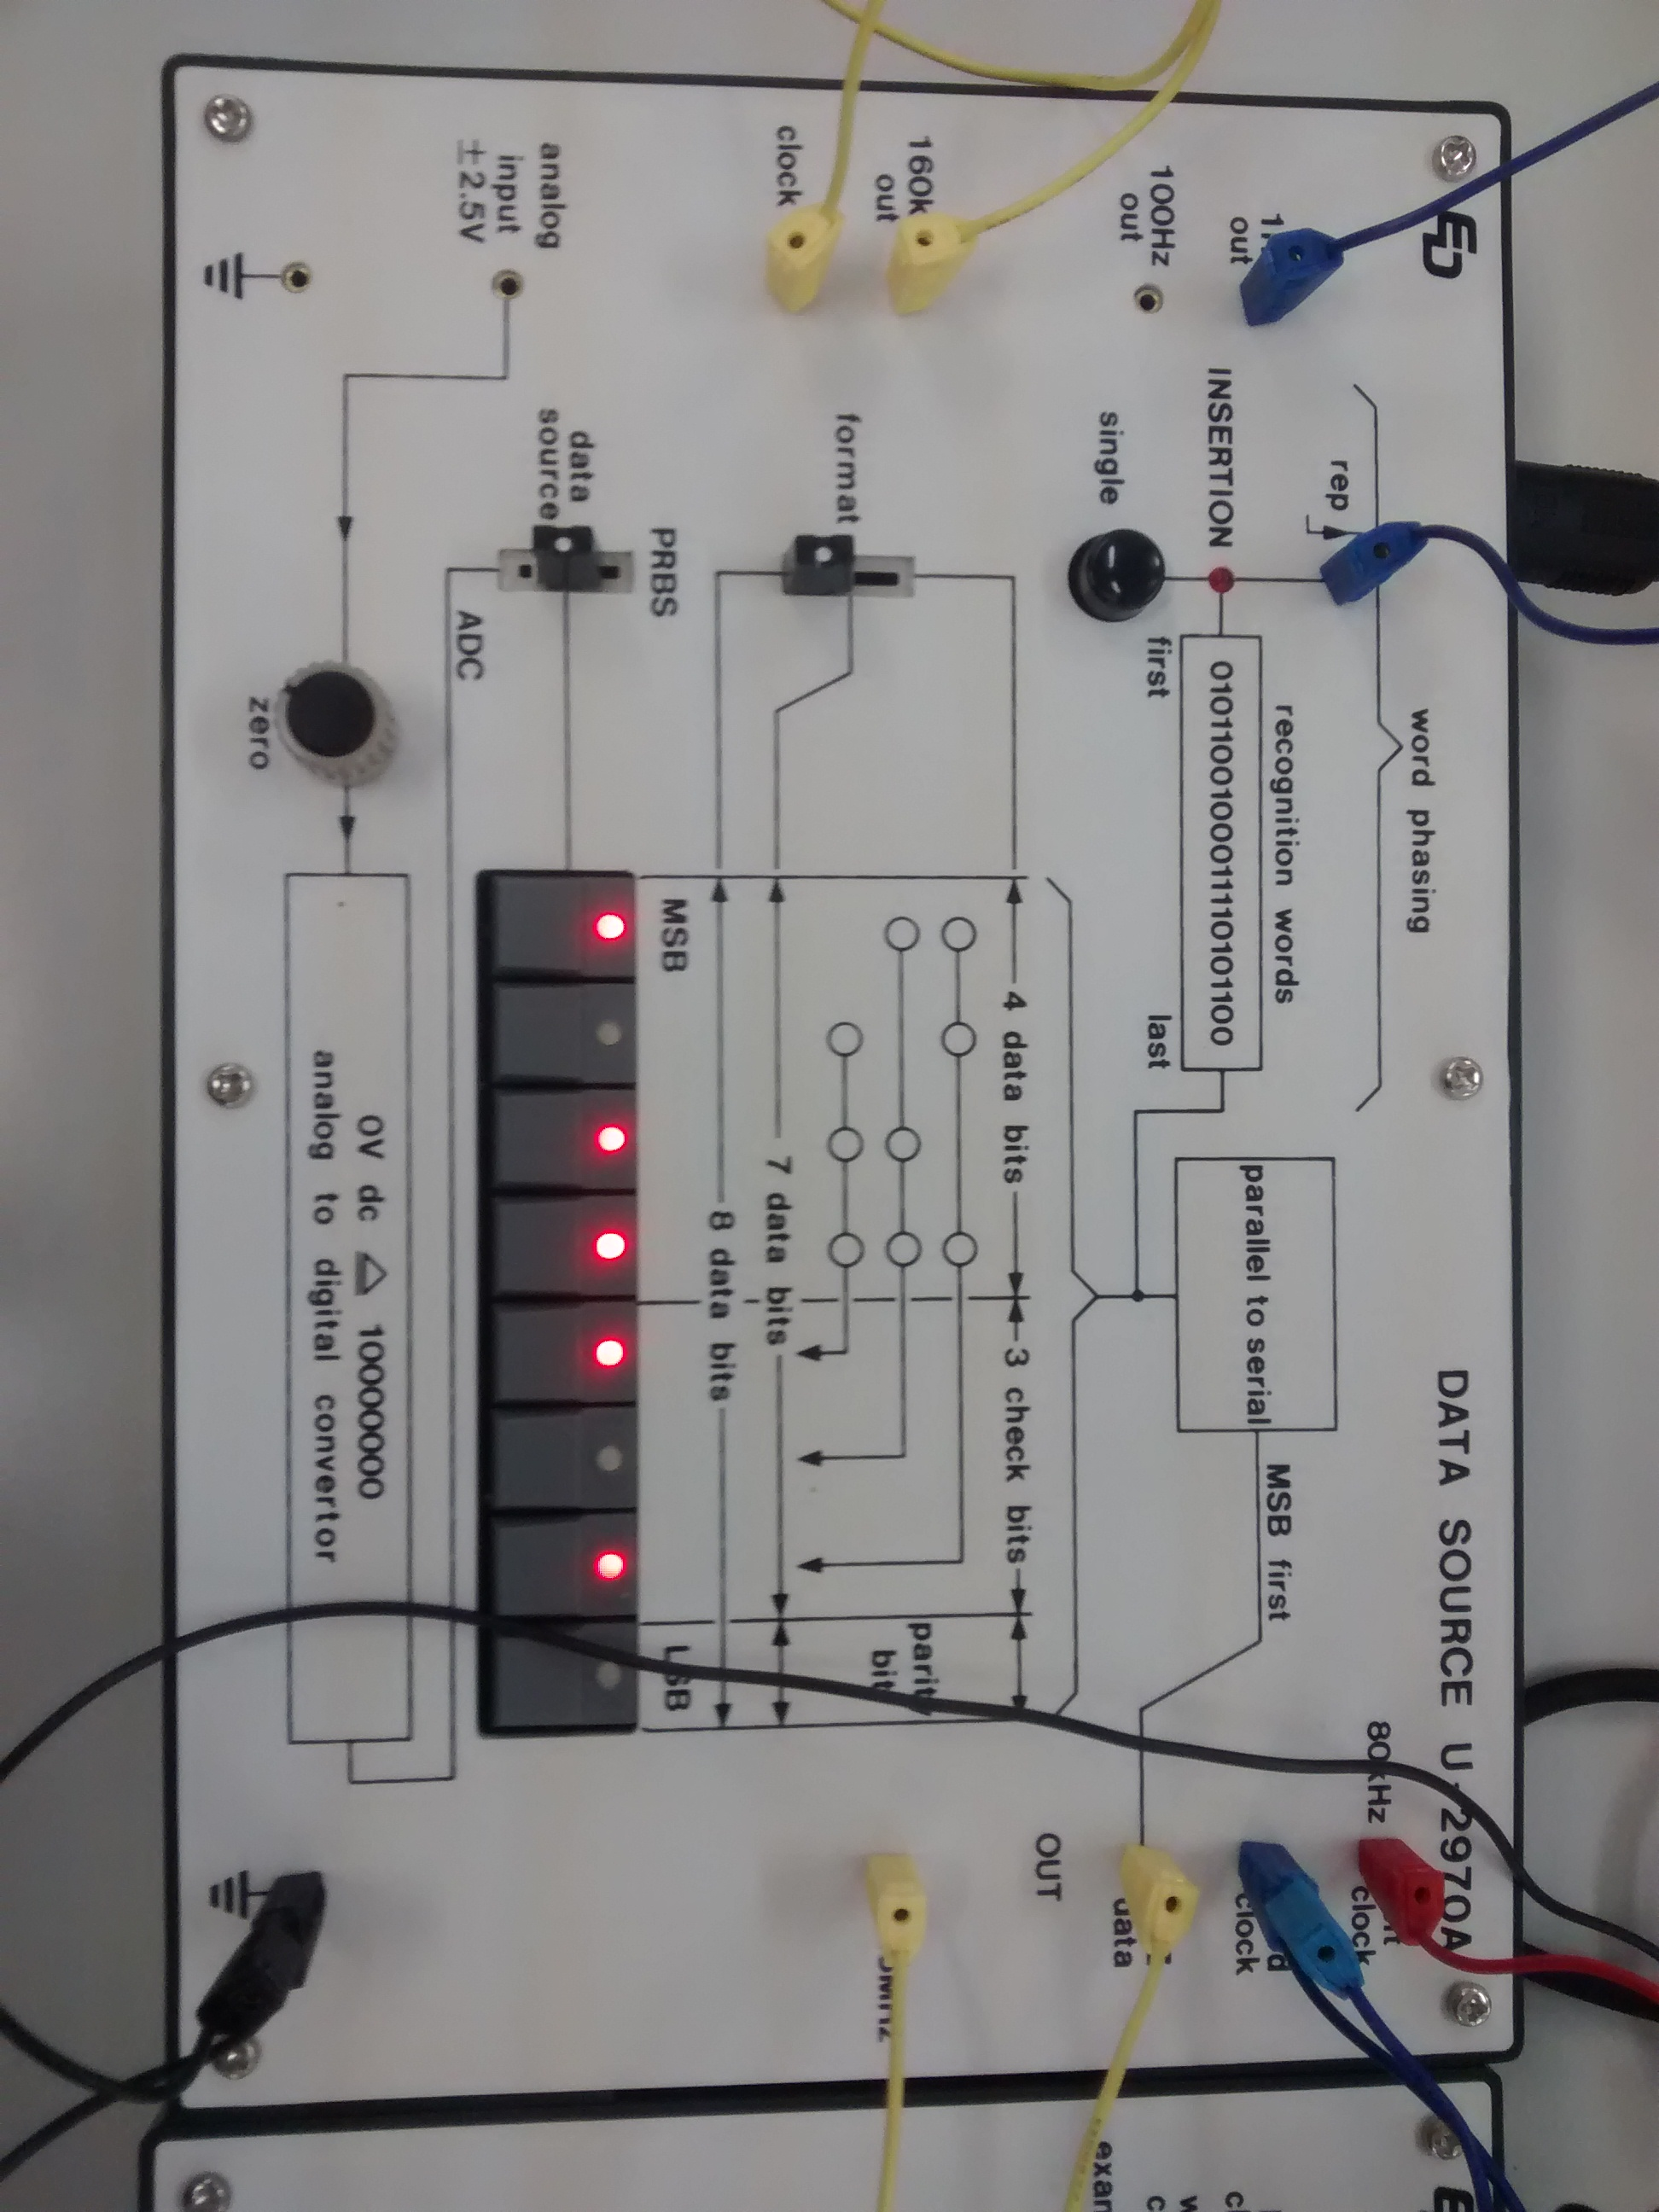
\includegraphics[scale=0.8]{montagem1}
  
  \small Fonte: Autoria própria.
  \label{fig:montagem1}
\end{figure}

Em seguida foram examinas as formas de onda para o sinal \emph{A} e \emph{B}, onde foi constatado que a onda \emph{A} possui os bits ímpares e a onda \emph{B} possui os bits pares, conforme mostram as figuras \ref{fig:osc1} e \ref{fig:osc2}, respectivamente.

\begin{figure}[H]
  \centering
  \caption{Forma de onda \emph{A}.}
  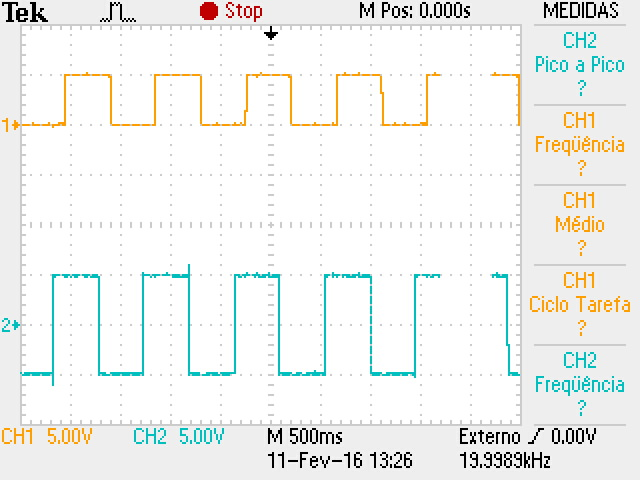
\includegraphics[scale=0.8]{osc1}
  
  \small Fonte: Autoria própria.
  \label{fig:osc1}
\end{figure}

\begin{figure}[H]
  \centering
  \caption{Forma de onda \emph{B}.}
  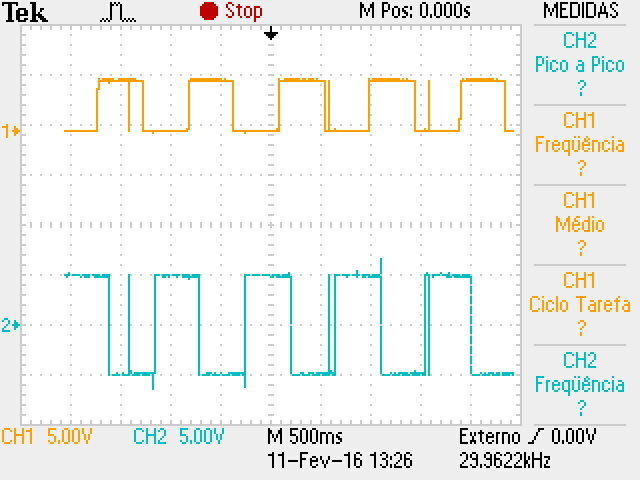
\includegraphics[scale=0.8]{osc2}
  
  \small Fonte: Autoria própria.
  \label{fig:osc2}
\end{figure}

Foi então investigada as formas de onda nos integradores \emph{A} e \emph{B}, conforme mostram as figuras \ref{fig:osc3} e \ref{fig:osc4}, respectivamente.

\begin{figure}[H]
  \centering
  \caption{Forma de onda do integrador \emph{A}.}
  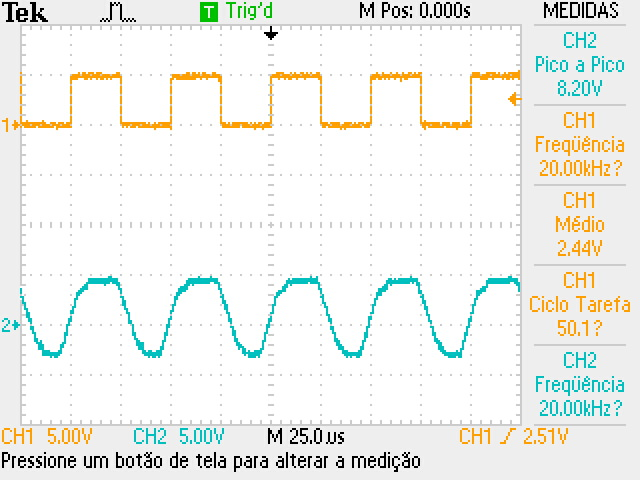
\includegraphics[scale=0.8]{osc4}
  
  \small Fonte: Autoria própria.
  \label{fig:osc3}
\end{figure}

\begin{figure}[H]
  \centering
  \caption{Forma de onda do integrador \emph{B}.}
  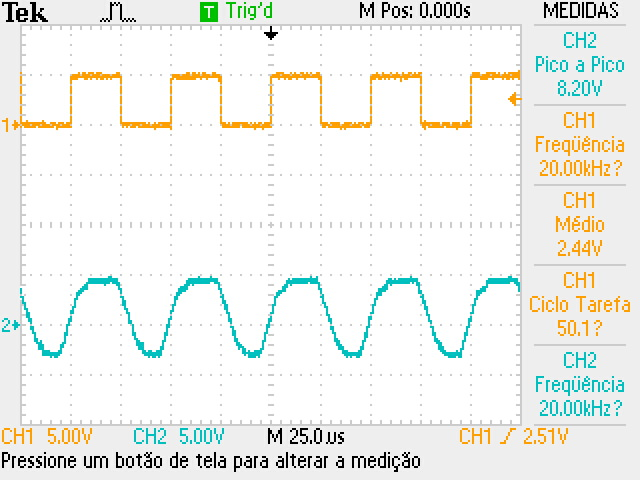
\includegraphics[scale=0.8]{osc4}
  
  \small Fonte: Autoria própria.
  \label{fig:osc4}
\end{figure}

Observou-se que a palavra é deslocada quando interrompemos o bit de clock. Também notou-se que a lampada A pisca para sinalizar o reconhecimento do deslocamento de palavra.

A montagem final é mostrada na figura \ref{fig:montagem2}.

\begin{figure}[H]
  \centering
  \caption{Montagem resultante para o primeiro experimento.}
  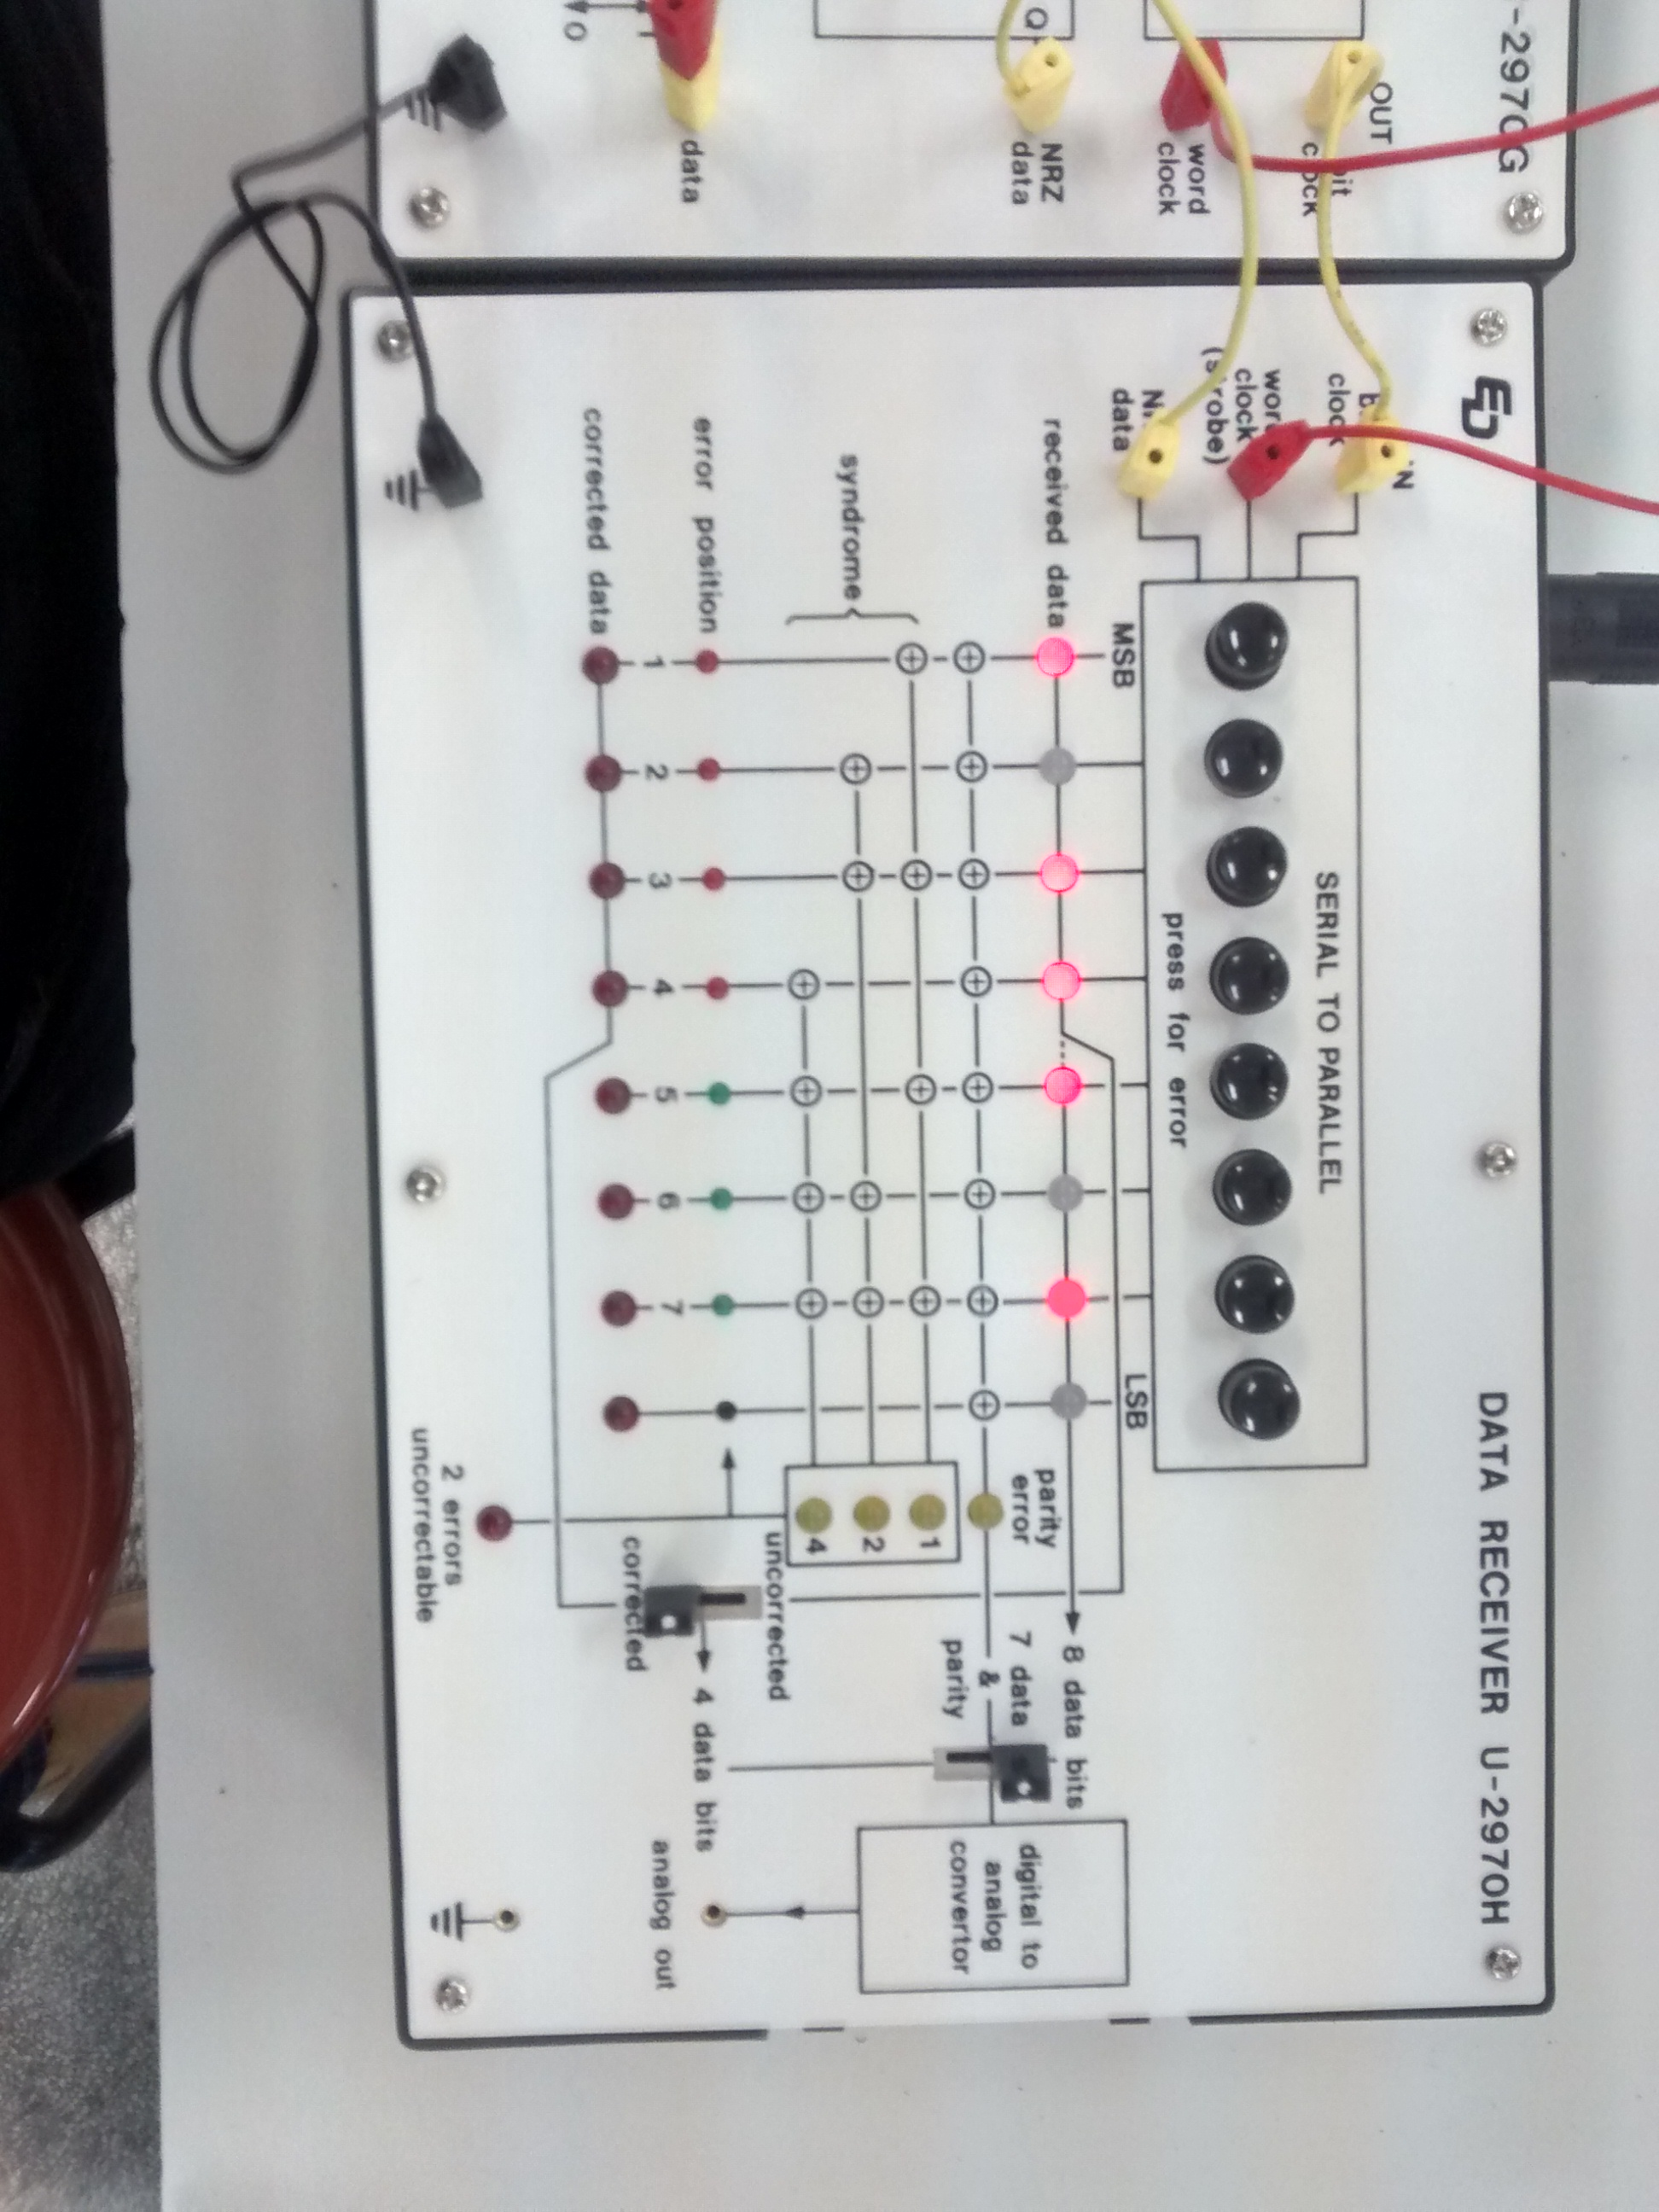
\includegraphics[scale=0.8]{montagem2}
  
  \small Fonte: Autoria própria.
  \label{fig:montagem2}
\end{figure}

\subsection{Método 2: Transmissão QSPK}

Para o método 2, primeiramente foi realizada a montagem, de acordo com a figura \ref{fig:montagem}-b, conforme mostra a figura \ref{fig:montagem3}.

\begin{figure}[H]
  \centering
  \caption{Montagem para o segundo experimento.}
  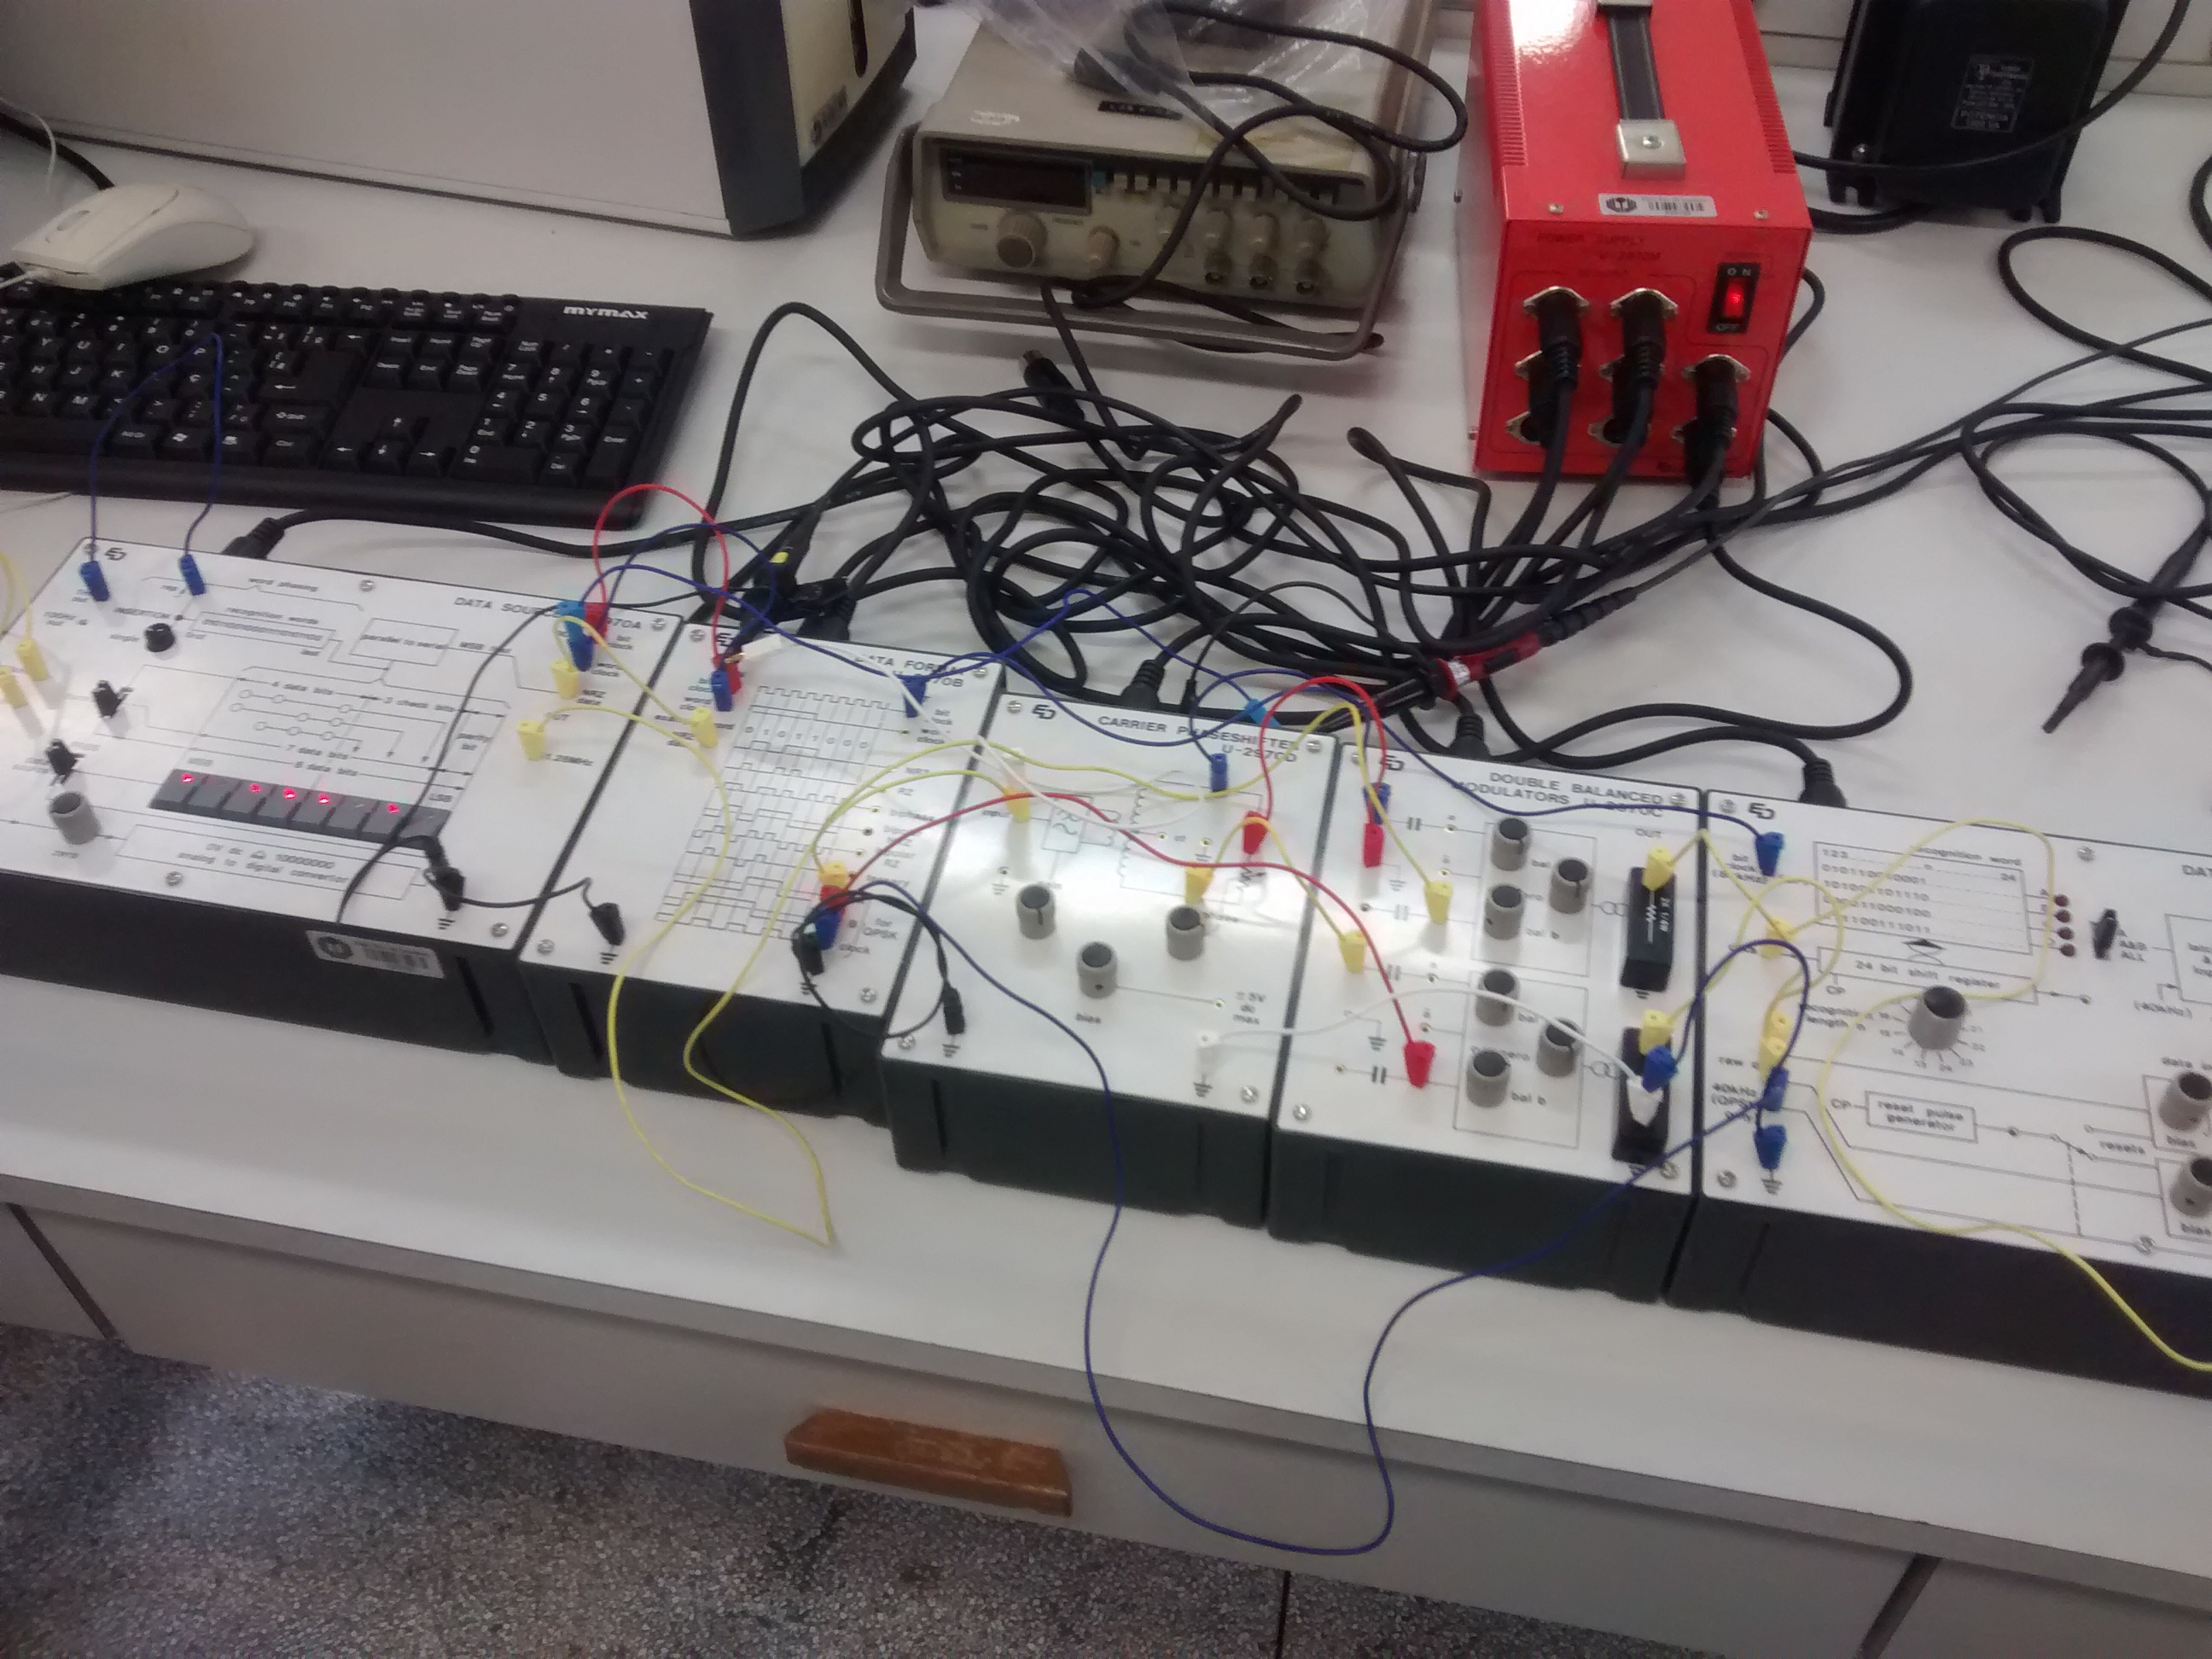
\includegraphics[scale=0.8]{montagem3}
  
  \small Fonte: Autoria própria.
  \label{fig:montagem3}
\end{figure}

Em seguida foi observado que os sinais estavam em quadratura, conforme mostra a figura \ref{fig:osc5}.

\begin{figure}[H]
  \centering
  \caption{Sinais em quadratura.}
  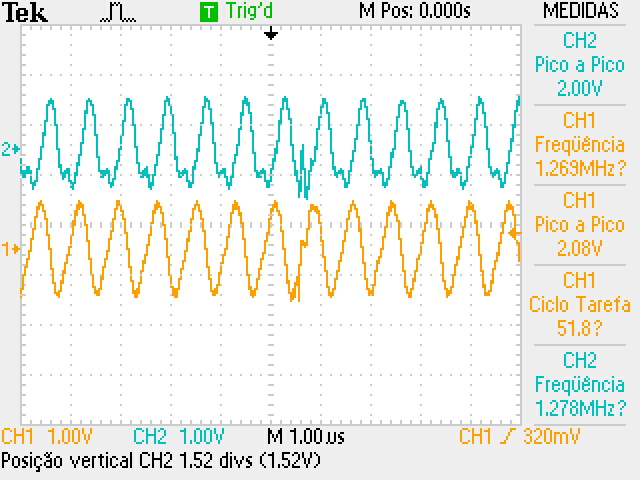
\includegraphics[scale=0.8]{osc5}
  
  \small Fonte: Autoria própria.
  \label{fig:osc5}
\end{figure}

Foram realizados os ajustes na montagem, como indicam os procedimentos 3 e 4. Observou-se que as duas senoides estavam em quadratura, como mostra a figura \ref{fig:osc6}.

\begin{figure}[H]
  \centering
  \caption{Senoides em quadratura.}
  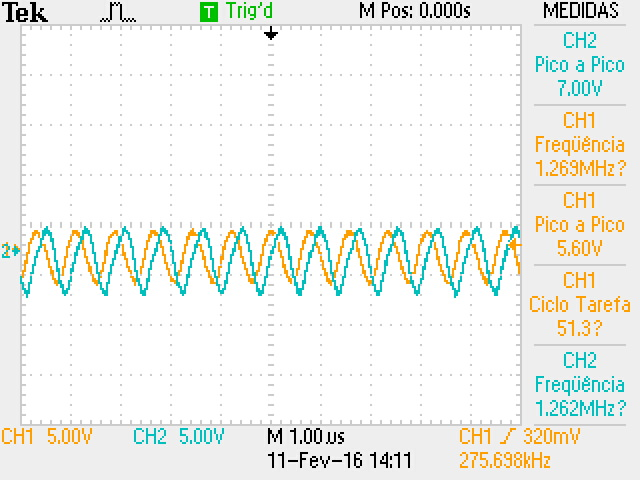
\includegraphics[scale=0.8]{osc6}
  
  \small Fonte: Autoria própria.
  \label{fig:osc6}
\end{figure}

Após as modificações dos itens 6 e 7, observou-se que a combinação impar muda o brilho do modulador superior e que a combinação par inverte a fase do modulador inferior.

Para visualizar a inversão de fase, os primeiros bits foram colocados em 00 (figura \ref{fig:osc7}) e em seguida em 11 (figura \ref{fig:osc8}). Fica evidente a inversão de fases.

\begin{figure}[H]
  \centering
  \caption{Bits 00000000.}
  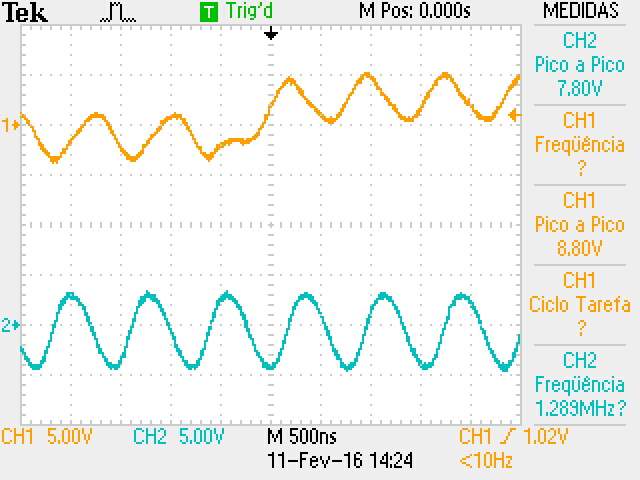
\includegraphics[scale=0.8]{osc7}
  
  \small Fonte: Autoria própria.
  \label{fig:osc7}
\end{figure}

\begin{figure}[H]
  \centering
  \caption{Bits 11000000.}
  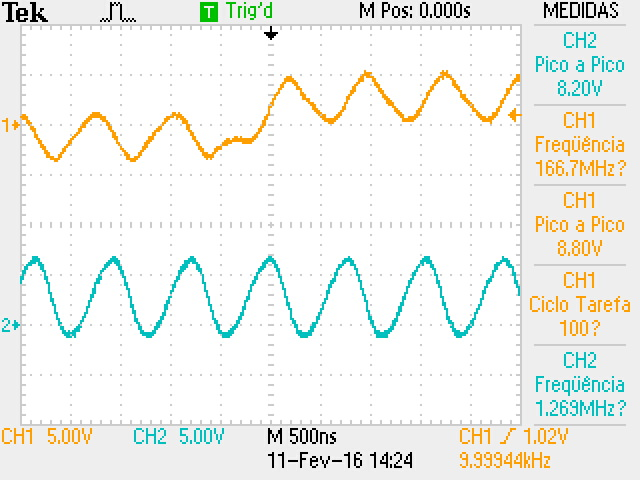
\includegraphics[scale=0.8]{osc8}
  
  \small Fonte: Autoria própria.
  \label{fig:osc8}
\end{figure}

Após as mudanças necessárias (itens 8-11) foram observados os sinais em 4 configurações diferentes, mostrados nas figuras \ref{fig:osc9}, \ref{fig:osc10}, \ref{fig:osc11} e \ref{fig:osc12}.

\begin{figure}[H]
  \centering
  \caption{Bits 00000000.}
  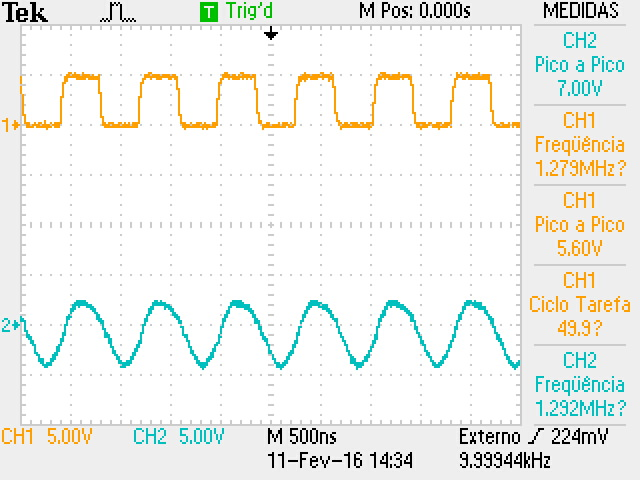
\includegraphics[scale=0.8]{osc9}
  
  \small Fonte: Autoria própria.
  \label{fig:osc9}
\end{figure}

\begin{figure}[H]
  \centering
  \caption{Bits 11111111.}
  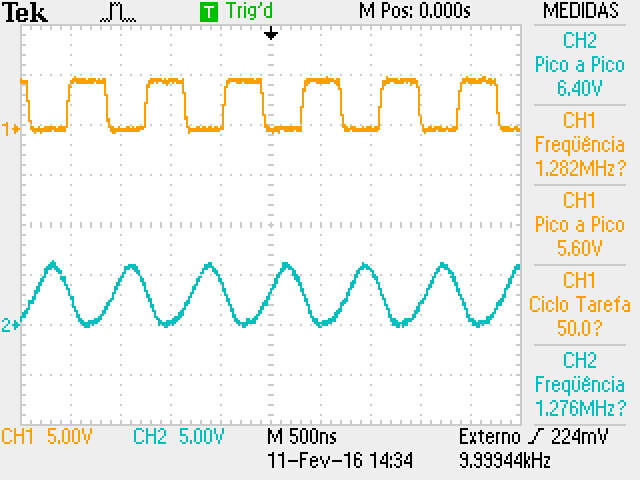
\includegraphics[scale=0.8]{osc10}
  
  \small Fonte: Autoria própria.
  \label{fig:osc10}
\end{figure}

\begin{figure}[H]
  \centering
  \caption{Bits 01010101.}
  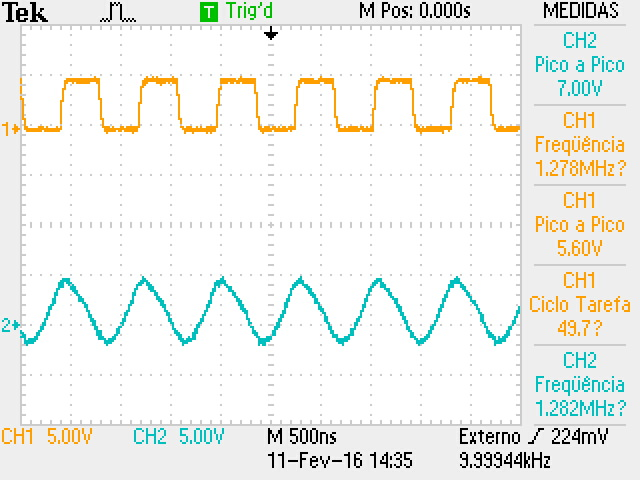
\includegraphics[scale=0.8]{osc11}
  
  \small Fonte: Autoria própria.
  \label{fig:osc11}
\end{figure}

\begin{figure}[H]
  \centering
  \caption{Bits 10101010.}
  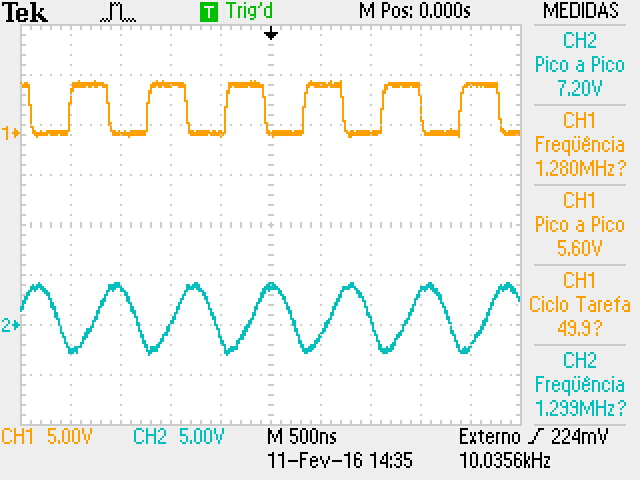
\includegraphics[scale=0.8]{osc12}
  
  \small Fonte: Autoria própria.
  \label{fig:osc12}
\end{figure}

Foi possível ver a forma de onda de saída que passando ciclicamente através de todas as suas quatro fases possíveis.

A figura \ref{fig:montagem4} mostra como ficou a montagem final.

\begin{figure}[H]
  \centering
  \caption{Montagem resultante para o segundo experimento.}
  \includegraphics[scale=0.8]{montagem4}
  
  \small Fonte: Autoria própria.
  \label{fig:montagem4}
\end{figure}

Por ultimo, a tabela \ref{tab:fases} mostra a relação entre o parte bits de dados e a fase das ondas, relativa a referência do canal 1 do osciloscópio.

\begin{table}[H]
  \centering
  \caption{Relação entre par de bits e fase.}
  \label{tab:fases}
  \begin{tabular}{cc}
    \toprule
    Bits & Fase [°] \\
    \midrule
    00 & 45 \\
    01 & 135 \\
    10 & 315 \\
    11 & 225 \\
    \bottomrule
  \end{tabular}
  
  \small Fonte: Autoria própria.
\end{table}

\newpage
\section{Discussão e Conclusão}
Neste experimento foi possível analisar o projeto de três topologias de circuitos adaptadores de impedância, onde foi possível constatar que, de fato, a potência transferida da fonte para a carga é maior com os mesmos.
Um dos fatores importantes observado foi a largura de banda diminui conforme o fator Q, porém, isso pode ser contornado com a utilização de redes do tipo $L$ em cascata ($L_{wideband}$).
Notório também é a diferença de qualidade, entre a rede $L$ simples e a rede $T$, onde a rede $T$ apresenta melhores resultados, a custa de componentes extras.
\newpage
\section{Referências}

[1] Roteiro da atividade prática.
\vspace{0.5cm}

[2] "Active Filter Design Techniques". Kugelstad, THomas. AmpOps For Everyone, Texas Instruments, 2008.
\vspace{0.5cm}

[3] "Electronic Devices and Circuit Theory, 11th ed.".  Robert L. Boylestad,11th 2006, Prentice Hall .


\end{document}